\documentclass{scrartcl}
\usepackage[a4paper,margin=2cm,footskip=1cm]{geometry}
\setkomafont{disposition}{\normalfont\bfseries}

%\documentclass{article}

\usepackage[table,xcdraw]{xcolor}
\usepackage{tikz}
\usetikzlibrary{angles,quotes}
\usetikzlibrary{babel}

\usepackage{booktabs}
\usepackage[utf8]{inputenc}
\usepackage[spanish, es-nodecimaldot]{babel}
\usepackage[per-mode=symbol]{siunitx}
\usepackage{graphicx}
\usepackage{subcaption}
\usepackage{caption}
\usepackage{mathtools}
\usepackage{amsmath}
\usepackage{slashed}
\usepackage{dsfont}
\usepackage{float}
\usepackage{multicol}
\usepackage{wrapfig}
\usepackage{lipsum}
\usepackage{textcomp}
\usepackage{gensymb}
\usepackage{longtable}
\usepackage{supertabular}
\usepackage{hhline}
\usepackage{enumerate}
\usepackage{multirow}
\usepackage{amssymb}
\usepackage{tabularx}
\usepackage{ragged2e}
\usepackage{rotating}
\usepackage{cancel}
\usepackage{physics}
\usepackage[framemethod=default]{mdframed}
\usepackage{csquotes}
%\usepackage[backend=biber, style=numeric, sorting=none]{biblatex}
\usepackage{qcircuit}
\usepackage{bm}

\renewcommand{\figurename}{Figura}
\renewcommand{\spanishtablename}{Tabla}
\newcommand{\inv}[1]{\frac{1}{#1}}
\newcommand{\uv}[1]{\hat{\mathbf{#1}}}
\newcommand{\uvs}[1]{\, \uv{#1}}

\newcommand{\realSet}{\mathbb{R}}
\newcommand{\complexSet}{\mathbb{C}}
\newcommand{\oref}{$\mathcal{O}$ }
\newcommand{\opref}{$\mathcal{O}'$ }
\newcommand{\oppref}{$\mathcal{O}''$ }

\def\residue{\mathop{\text{Res}}}

\setlength{\tabcolsep}{19pt}

\DeclareSIUnit\clight{\text{\ensuremath{c}}}
\DeclareSIUnit\MeV{\mega\electronvolt}
\DeclareSIUnit\GeV{\giga\electronvolt}
\DeclareSIUnit\MeVpc{\MeV\per\clight\squared}
\DeclareSIUnit\GeVpc{\GeV\per\clight\squared}

\newcommand{\sinc}{\text{sinc}}
\newcommand{\E}{\vb{E}}
\newcommand{\B}{\vb{B}}
\newcommand{\x}{\vb{x}}
\newcommand{\y}{\vb{y}}
\newcommand{\z}{\vb{z}}
\newcommand{\p}{\vb{p}}
\renewcommand{\k}{\vb{k}}
\newcommand{\Lag}{\mathcal{L}}
\newcommand{\Ham}{\mathcal{H}}

\newcommand{\tx}{\tilde{x}}

\renewcommand{\vb}[1]{\bm{#1}}

\renewcommand{\a}[1]{\hat{a}_{#1}}
\newcommand{\ad}[1]{\hat{a}_{#1}^\dagger}

\DeclareRobustCommand{\[}{\begin{equation}}
\DeclareRobustCommand{\]}{\end{equation}}
\mathtoolsset{showonlyrefs}

\allowdisplaybreaks

%\bibliography{bibliography}

%----------------------------------------------------------------------------------------
%	DOCUMENT INFORMATION
%----------------------------------------------------------------------------------------

\title{Teoría de la Información Cuántica}
\subtitle{Práctica 5 - Año 2020}
\author{\textsc{Beaucamp}, Jean Yves}
\date{}

\begin{document}

\maketitle

\section{Transformada de Fourier Cuántica}
\begin{enumerate}
    
    %-------------------------------------------------------------------------------------------------------
    %   Problema 1
    %-------------------------------------------------------------------------------------------------------
    \item Consideremos la transformada de Fourier discreta de un conjunto de $N$ números ($f_j \in \complexSet$, $j = 0, 1, \dots, N-1$), dada por
    \[  F_k = \inv{\sqrt{N}} \sum_{j = 0}^{N-1} f_j e^{-i\frac{2\pi}{N} jk}. \]
    
    \begin{enumerate}
        \item La transformada de Fourier discreta inversa se encuentra determinada por
        \[ f_j = \inv{\sqrt{N}} \sum_{k = 0}^{N-1} F_k e^{i\frac{2\pi}{N} jk}, \quad \quad j = 0, 1, \dots, N - 1, \]
        satisfaciendo la identidad $\mathcal{F}[\mathcal{F}^{-1}[F_{k'}]]_k = F_k$:
        \begin{align}
            \mathcal{F}[f_j]_k &= \inv{\sqrt{N}} \sum_{j = 0}^{N-1} \left[ \inv{\sqrt{N}} \sum_{k' = 0}^{N-1} F_{k'} e^{i\frac{2\pi}{N} jk'} \right] e^{-i\frac{2\pi}{N} jk} \\
                &= \inv{N} \sum_{j = 0}^{N-1} \sum_{k' = 0}^{N-1} F_{k'} e^{i\frac{2\pi}{N} jk'} e^{-i\frac{2\pi}{N} jk} \\
                &= \inv{N} \sum_{k' = 0}^{N-1} F_{k'} \sum_{j = 0}^{N-1} e^{-i\frac{2\pi}{N} j (k-k')}. \label{eq:1_a_1}
        \end{align}
        Luego, si $k = k'$, entonces
        \[ \sum_{j = 0}^{N - 1} e^{i \frac{2\pi}{N} j 0} = \sum_{j = 0}^{N - 1} 1 = N, \]
        mientras que para $k \neq k'$, como $k - k' = m \in \mathds{Z}$,
        \[ \sum_{j = 0}^{N - 1} e^{i \frac{2\pi}{N} j (k - k')} = \sum_{j = 0}^{N - 1} \qty(e^{i \frac{2m\pi}{N}})^j = \frac{1 - e^{i \frac{2m\pi}{N} N}}{1 - e^{i \frac{2m\pi}{N}}} = \frac{1 - e^{i 2m\pi}}{1 - e^{i \frac{2m\pi}{N}}} = \frac{1 - 1}{1 - e^{i \frac{2m\pi}{N}}} = 0. \]
        Podemos escribir estos resultados de manera compacta como,
        \[ \sum_{j = 0}^{N - 1} e^{i \frac{2\pi}{N} j (k - k')} = N \delta_{k k'}, \]
        con lo que \eqref{eq:1_a_1} resulta en
        \[ \mathcal{F}[f_j]_k = \inv{N} \sum_{k' = 0}^{N-1} F_{k'} N \delta_{k k'} = F_k. \]
        
        
        \item Si extendemos el conjunto de posibles valores de $k$ a todo $k \in \mathds{Z}$ en la definición de la TF discreta, es fácil ver que
        \[ F_{k + lN} = \inv{\sqrt{N}} \sum_{j = 0}^{N-1} f_j e^{-i\frac{2\pi}{N} j (k + lN)} = \inv{\sqrt{N}} \sum_{j = 0}^{N-1} f_j e^{-i\frac{2\pi}{N} jk} e^{-i2\pi jl} = \inv{\sqrt{N}} \sum_{j = 0}^{N-1} f_j e^{-i\frac{2\pi}{N} jk} = F_k. \]
        
        
        \item Si $f_j$ es una función periódica con período $r$, tal que $f_{j + r} = f_{j}$, con $r | N$ ($r$ divisor de $N$), entonces escribiendo a $f_j$ como la anti-transformada de Fourier de $F_k$ vemos que
        \[ f_{j} = f_{j + r} \iff \inv{N} \sum_{k = 0}^{N - 1} F_k e^{i \frac{2\pi}{N} jk} = \inv{N} \sum_{k = 0}^{N - 1} F_k e^{i \frac{2\pi}{N} (j + r) k} \]
        \[ \implies F_k = 0 \forall k = 0, \dots N-1, \quad \vee e^{i \frac{2\pi}{N} rk}. \]
        El segundo caso se reduce fácilmente a la condición
        \[ \frac{rk}{N} = m \in \mathds{Z} \implies k = m \frac{N}{r} \iff \frac{N}{r} | k. \]
        
        Más aún, si $k = m N/r$, entonces
        \[ F_k = \inv{\sqrt{N}} \sum_{j = 0}^{N - 1} f_j e^{-i \frac{2\pi}{N} jk} = \inv{\sqrt{N}} \sum_{j = 0}^{N - 1} f_j e^{-i \frac{2\pi}{N} j \frac{mN}{r}} = \inv{\sqrt{N}} \sum_{j = 0}^{N - 1} f_j e^{-i 2\pi \frac{jm}{r}}. \]
        Siguiendo los pasos de 1.b, es fácil ver que la exponencial con su argumento así definido resulta periódica en $r$, con lo que considerando que $f_j$ es también de período $r$, podemos concluir que todo el sumando es una función periódica de período $r$. Por lo tanto, como $r | N$, entonces podremos separar la sumatoria en $N/r$ partes iguales, resultando en
        \[ F_k = \inv{\sqrt{N}} \sum_{j = 0}^{N - 1} f_j e^{-i 2\pi \frac{jm}{r}} = \inv{\sqrt{N}} \frac{N}{r} \sum_{j = 0}^{r - 1} f_j e^{-i 2\pi \frac{jm}{r}} = \frac{\sqrt{N}}{r} \sum_{j = 0}^{r - 1} f_j e^{-i 2\pi \frac{jm}{r}}. \]
        
    \end{enumerate}
    
    
    
    %-------------------------------------------------------------------------------------------------------
    %   Problema 2
    %-------------------------------------------------------------------------------------------------------
    \item Sea $\displaystyle f_j = \inv{\sqrt{N}} e^{i \frac{2\pi}{N} xj}$. Su transformada discreta de Fourier resultará en
    \[ F_k = \inv{\sqrt{N}} \sum_{j = 0}^{N - 1} \inv{\sqrt{N}} e^{i \frac{2\pi}{N} xj} e^{-i \frac{2\pi}{N} jk} = \inv{N} \sum_{j = 0}^{N - 1} e^{i \frac{2\pi}{N} (x - k) j}. \]
    Suponiendo que $x \neq k$, entonces aplicando la fórmula de suma de una serie parcial geométrica,
    \begin{align}
        F_k = \inv{N} \frac{1 - e^{i \frac{2\pi}{N} (x - k) N}}{1 - e^{i \frac{2\pi}{N} (x - k)}} &= \inv{N} \frac{e^{i \pi (x - k)}}{e^{i \frac{\pi}{N} (x - k)}} \frac{e^{-i \pi (x - k)} - e^{i \pi (x - k)}}{e^{-i \frac{\pi}{N} (x - k)} - e^{i \frac{\pi}{N} (x - k)}} \\
            &= \inv{N} e^{i \pi (x - k) (1 - 1/N)} \frac{\sin[\pi (x - k)]}{\sin[\pi (x - k) / N]}.
    \end{align}
    Luego, como el argumento de la exponencial remanente en el último término de la igualdad es un número puramente imaginario,
    \[ \abs{F_k} = \abs{\frac{\sin[\pi (x - k)]}{N \sin[\pi (x - k) / N]}} = \abs{\frac{\sinc[\pi (x - k)]}{\sinc[\pi (x - k) / N]}}. \label{eq:2_a_1} \]
    
    Si $x \in \mathds{Z}$, para $0 \neq \abs{k - x} < N$, el denominador de \eqref{eq:2_a_1} resulta no-nulo, mientras que el argumento de la función seno cardinal del numerador resulta un múltiplo entero de $\pi$, por lo que $F_k = 0$. Por el contrario, para $k = x$, $F_x = 1$. El caso en que $k - x = \pm N$, evaluando la función en el límite (extendiendo $F_k$ al dominio continuo, como $F(k)$) obtenemos
    \[ \lim_{k - x \to N} F_k = 1. \]
    Por lo tanto, para $x \in \mathds{Z}$, $F_k = \delta_{(k - x) \mod N = 0}$, reduciéndose para $\abs{k} < N$ a $F_k = \delta_{k x}$.
    
    Si, por el contrario, permitimos $x \not\in \mathds{Z}$, entonces $F_k$ presentará un comportamiento asintótico a $\delta_{(k - x) \mod N = 0}$ en el límite $N \to \infty$, aunque resultará no nula para $(k - x) \mod N \neq 0$, intersectando las oscilaciones de la función continua $F(k)$, como podemos observar en la fig. \ref{fig:2_b}.
    
    Es claro que, como $F(k)$ posee un máximo en $k - x \mod N = 0$ (en el intervalo $0 < k < N - 1$), por lo que $F_k$ tendrá un máximo en el entero $k \in \mathds{Z}$ más próximo a $x$.
    
    \begin{figure}[t]
        \centering
        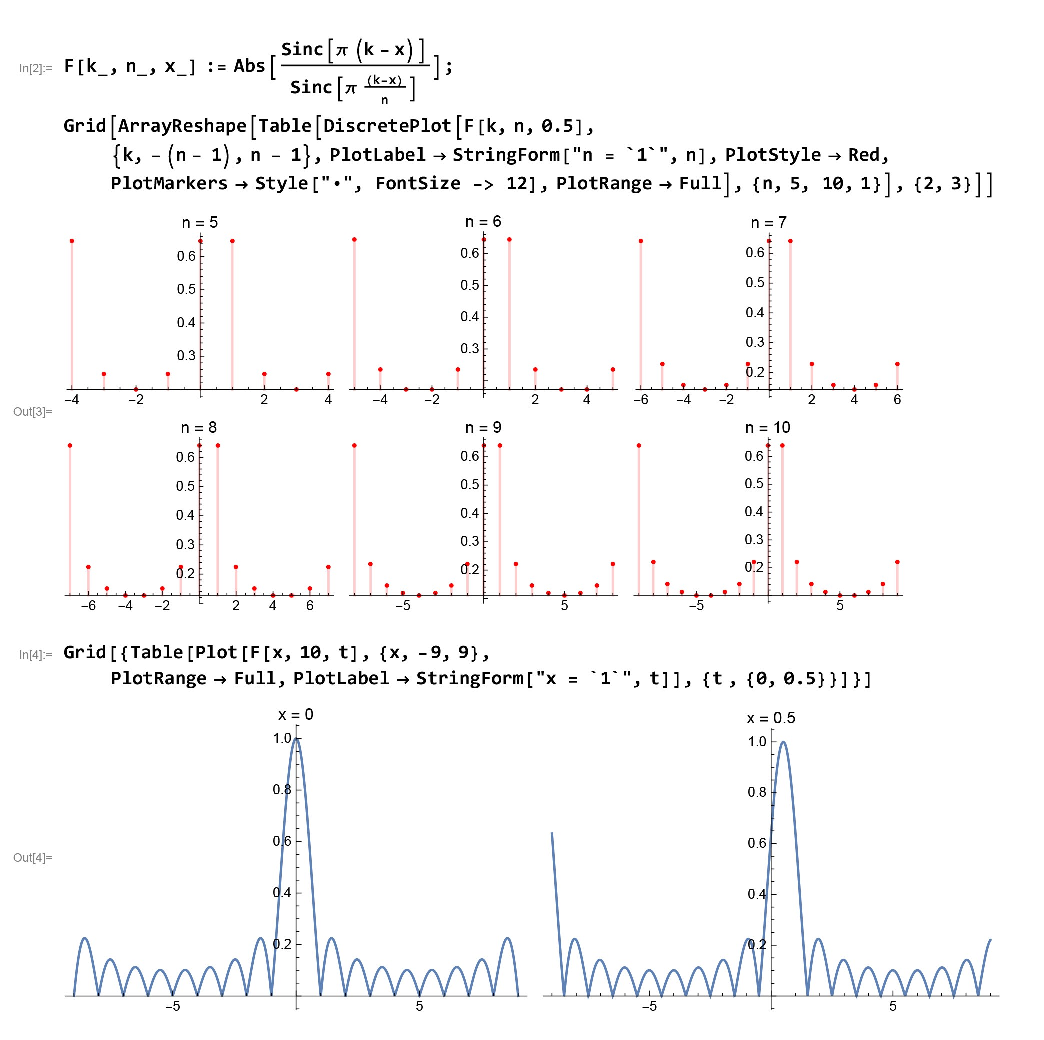
\includegraphics[width=\linewidth]{Images/2.pdf}
        \caption{}
        \label{fig:2_b}
    \end{figure}
    
    
    
    %-------------------------------------------------------------------------------------------------------
    %   Problema 3
    %-------------------------------------------------------------------------------------------------------
    \item \begin{enumerate}
        \item Sea $\{ \ket{j}, j = 0, \dots, N-1 \}$ una base ortonormal de un espacio $V$. Definimos la Transformada de Fourier cuántica de $\ket{k}$ como la operación $\hat U$:
        \[ \ket{\tilde{k}} = \hat{U} \ket{k} = \inv{N} \sum_{j = 0}^{N - 1} e^{i \frac{2\pi}{N} kj} \ket{j}, \quad \quad k = 0, 1, \dots, N - 1. \]
        
        Es fácil ver que los estados $\{ \ket{\tilde{k}} \}$ forman también una base ortonormal, escribiendo
        \[ \ip{\tilde{k}}{\tilde{k}'} = \mel{k'}{\hat U^\dagger \hat U}{k} = \inv{N} \sum_{j, j' = 0}^{N-1} e^{i \frac{2\pi}{N} (kj - k'j')} \ip{j'}{j} = \inv{N} \sum_{j, j' = 0}^{N-1} e^{i \frac{2\pi}{N} j (k - k')} = \delta_{k k'}, \]
        \[ \implies \hat U^\dagger \hat U = \mathds{1}. \]
        Por un tratamiento análogo con las transformadas de Fourier cuánticas inversas se puede probar también que $\hat U \hat U^\dagger = \mathds{1}$, quedando demostrado que la operación $\hat U$ es unitaria.
        
        
        \item Sea un estado $\ket{\psi} = \sum_{j = 0}^{N - 1} c_j \ket{j}$. Al ser $\{ \ket{\tilde{k}} \}$ también una base ortonormal de $V$, podremos describir a $\ket{\psi}$ también en términos de $\ket{\tilde{k}}$ como $\psi = \sum_{k = 0}^{N - 1} C_k \ket{\tilde{k}}$. La relación entre $c_j$ y $C_k$ puede ser determinada a partir de las condiciones de ortonormalidad de las bases, como
        \[ \ip{\tilde{k}}{\psi} = \sum_{k' = 0}^{N - 1} C_{k'} \ip{\tilde{k}}{\tilde{k}'} = C_k = \sum_{j = 0}^{N - 1} c_j \left( \inv{\sqrt{N}} \sum_{j' = 0}^{N - 1} e^{-i \frac{2\pi}{N} j' k} \bra{j'}\right) \ket{j} = \inv{\sqrt{N}} \sum_{j = 0}^{N - 1} c_j e^{-i \frac{2\pi}{N} j k} \]
        \[ \therefore C_k = \inv{\sqrt{N}} \sum_{j = 0}^{N - 1} c_j e^{-i \frac{2\pi}{N} j k}. \]
        
        
        \item Sean $\hat X$, $\hat P$, y $\hat T$ operadores definidos por $\hat X \ket{j} = j \ket{j}$, $\hat P = \hat U \hat X \hat U^\dagger$, y $\hat T = e^{-i \frac{2\pi}{N} \hat P}$. Entonces,
        \[ \hat P \ket{\tilde{k}} = \hat U \hat X \hat U^\dagger \ket{\tilde{k}} = \hat U \hat X \underbrace{\hat U^\dagger \hat U}_{= \mathds{1}} \ket{k} = \hat U \hat X \ket{k} = k \hat U \ket{k} = k \ket{\tilde{k}}, \]
        \[ \hat T \ket{\tilde{k}} = \sum_{n = 0}^\infty \frac{\qty(-i \frac{2\pi}{N})^n}{n!} \hat P^n \ket{\tilde{k}} = = \sum_{n = 0}^\infty \frac{\qty(-i \frac{2\pi}{N})^n}{n!} k^n \ket{\tilde{k}} = e^{-i \frac{2\pi}{N} k} \ket{\tilde{k}}, \]
        y
        \begin{align}
            \hat T \ket{j} = \hat T \left( \inv{\sqrt{N}} \sum_{k = 0}^{N - 1} e^{-i \frac{2\pi}{N} jk} \ket{\tilde{k}} \right) = \inv{\sqrt{N}} \sum_{k = 0}^{N - 1} e^{-i \frac{2\pi}{N} jk} e^{-i \frac{2\pi}{N} k} \ket{\tilde{k}} &= \inv{\sqrt{N}} \sum_{k = 0}^{N - 1} e^{-i \frac{2\pi}{N} (j + 1)k} \ket{\tilde{k}} \\
                &= \ket{j + 1}.
        \end{align}
        
    \end{enumerate}
    
    
    
    %-------------------------------------------------------------------------------------------------------
    %   Problema 4
    %-------------------------------------------------------------------------------------------------------
    \item Sea $\ket{\tilde{k}}$ el estado transformado en Fourier de $\ket{j}$. En un sistema de $n$ qubits, $N = 2^n$, pudiendo describir a los estados $\ket{j}$ en términos de su descomposición en dígitos binaria como
    \[ j = j_1 2^{n - 1} + j_2 2^{2 - 2} + \dots j_n 2^0 = \sum_{l = 1}^n j_l 2^{n - l}. \]
    Luego,
    \begin{align}
        \ket{\tilde{k}} &= \inv{2^{n/2}} \sum_{j = 0}^{2^n - 1} e^{i \frac{2\pi}{2^n} kj} \ket{j} \\
            &= \inv{2^{n/2}} \sum_{j = 0}^{2^n - 1} e^{i \frac{2\pi}{2^n} k \sum_{l = 1}^n j_l 2^{n - l} } \ket{j} \\
            &= \inv{2^{n/2}} \sum_{j_1 = 0}^{1} \dots \sum_{j_n = 0}^{1} e^{i 2\pi k \sum_{l = 1}^n j_l 2^{-l} } \ket{j_1 j_2 \dots j_n} \\
            &= \inv{2^{n/2}} \sum_{j_1 = 0}^{1} \dots \sum_{j_n = 0}^{1} \bigotimes_{l = 1}^n e^{i 2\pi k j_l 2^{-l} } \ket{j_l} \\
            &= \inv{2^{n/2}} \bigotimes_{l = 1}^n \left[ \sum_{j_l = 0}^{1} e^{i 2\pi k j_l 2^{-l} } \ket{j_l} \right] \\
            &= \inv{2^{n/2}} \bigotimes_{l = 1}^n \left[ \ket{0} + e^{i 2\pi k / 2^l } \ket{1} \right].
    \end{align}
    
    Para un sistema de 1 qubit, esta resulta en
    \[ \ket{\tilde{k}} = \inv{\sqrt{2}} \left[ \ket{0} + e^{i \pi k } \ket{1} \right] = \inv{\sqrt{2}} \left[ \ket{0} + (-1)^k \ket{1} \right], \]
    siendo equivalente a la acción de una compuerta Haddamard 
    \[ H = \inv{\sqrt{2}} \begin{pmatrix} 1 & 1 \\ 1 & -1 \end{pmatrix} \]
    sobre el qubit original, representado por el circuito en la figura \ref{fig:4_1}.
    
    Para un sistema de 2 qubits, la transformada de Fourier será
    \begin{align}
        \ket{\tilde{k}} &= \inv{2} \left[ \ket{0} + e^{i \pi k } \ket{1} \right] \otimes \left[ \ket{0} + e^{i \pi k / 2 } \ket{1} \right] \\
            &= \inv{2} \left[ \ket{0} + (-1)^k \ket{1} \right] \otimes \left[ \ket{0} + e^{i \pi k / 2 } \ket{1} \right],
    \end{align}
    siendo representado por el circuito cuántico de la fig. \ref{fig:4_2}, donde la operación sobre el segundo qubit consiste en la composición de una compuerta Haddamard, y una rotación $R_2$ dada por
    \[ R_2 = \begin{pmatrix} 1 & 0 \\ 0 & e^{i \pi / 2} \end{pmatrix} = \begin{pmatrix} 1 & 0 \\ 0 & i \end{pmatrix}. \]
    
    
    \begin{figure}
        \centering
        \begin{subfigure}{\linewidth}
            \[
                \begin{array}{c}
                    \Qcircuit @C=1.4em @R=1.2em {
                        \lstick{\ket{k}} & \gate{QFT} & \rstick{\inv{\sqrt{2}} (\ket{0} + e^{i\pi k} \ket{1})} \qw \\
                    }
                \end{array}
                \quad \quad \quad \quad \quad \quad \quad
                =
                \quad \quad
                \begin{array}{c}
                    \Qcircuit @C=1.4em @R=1.2em {
                        \lstick{\ket{k}} & \gate{H} & \rstick{\inv{\sqrt{2}} (\ket{0} + e^{i\pi k} \ket{1})} \qw \\
                    }
                \end{array}
            \]
            \caption{}
            \label{fig:4_1}
        \end{subfigure}
        \begin{subfigure}{\linewidth}
            \[
                \begin{array}{c}
                    \Qcircuit @C=1.4em @R=1.2em {
                        \lstick{\ket{k_1}} & \multigate{1}{QFT} & \rstick{\inv{2} (\ket{0} + e^{i \pi k / 2} \ket{1})} \qw \\
                        \lstick{\ket{k_2}} & \ghost{QFT} & \rstick{\inv{2} (\ket{0} + e^{i\pi k} \ket{1})} \qw \\
                    }
                \end{array}
                \quad \quad \quad \quad \quad \quad \quad \quad
                =
                \quad \quad \;
                \begin{array}{c}
                    \Qcircuit @C=1.4em @R=1.2em {
                        \lstick{\ket{k_1}} & \gate{H} & \gate{R_2} & \qw & \rstick{\inv{2} (\ket{0} + e^{i \pi k / 2} \ket{1})} \qw \\
                        \lstick{\ket{k_2}} & \qw & \ctrl{-1} & \gate{H} & \rstick{\inv{2} (\ket{0} + e^{i\pi k} \ket{1})} \qw \\
                    }
                \end{array}
            \]
            \caption{}
            \label{fig:4_2}
        \end{subfigure}
        \caption{Circuitos del algoritmo de Transformada de Fourier Cuántica para un estado de (a) 1 qubit y (b) 2 qubits.}
        \label{fig:4}
    \end{figure}
    
    
    
    %-------------------------------------------------------------------------------------------------------
    %   Problema 5
    %-------------------------------------------------------------------------------------------------------
    \item \begin{enumerate}
        \item En general, los algoritmos cuánticos basados en la transformada de Fourier se componen del siguiente esquema:
        \begin{align}
            \ket{0}\ket{0} &\overset{\hat{H}^{\otimes^{2^t}}}{\longrightarrow} \inv{2^{n/2}} \sum_{j = 0}^{2^n - 1} \ket{j} \ket{0} \\
                &\overset{\hat{U}}{\longrightarrow} \inv{2^{n/2}} \sum_{j = 0}^{2^n - 1} \ket{j} \ket{f(j)} \\ %= \inv{2^n} \sum_{k = 0}^{2^n - 1} \ket{\tilde{k}} \sum_{j = 0}^{2^n - 1} e^{-i \frac{2\pi}{2^n} kj} \ket{f(j)} \\
                &\overset{FT^{-1}}{\longrightarrow} \inv{2^n} \sum_{k = 0}^{2^n - 1} \ket{k} \sum_{j = 0}^{2^n - 1} e^{-i \frac{2\pi}{2^n} kj} \ket{f(j)},
        \end{align}
        donde $\hat{U}$ es una operación sobre el último qubit (o conjunto de qubits, tal que contengan la información del sistema), controlada sobe el primer conjunto de n-qubits, y $FT^{-1}$ representa a la transformada de Fourier inversa.
        
        \item En el caso de estimación de fase, el estado transformado del segundo conjunto de qubits se encuentra descrito por $\ket{f(j)} = e^{i \frac{2\pi}{2^n} xj} \ket{\Phi}$, con $0 \leq x \leq 2^n$. Si $x = m \in \mathds{Z}$, con $0 \leq m \leq N - 1$, entonces el estado final del algoritmo de estimación de fase resultará en
        \begin{align}
            \inv{2^n} \sum_{k = 0}^{2^n - 1} \ket{k} \sum_{j = 0}^{2^n - 1} e^{-i \frac{2\pi}{2^n} kj} \ket{f(j)} &= \inv{2^n} \sum_{k = 0}^{2^n - 1} \ket{k} \sum_{j = 0}^{2^n - 1} e^{-i \frac{2\pi}{2^n} kj} e^{i \frac{2\pi}{2^n} mj} \ket{\Phi} \\
                &= \inv{2^n} \sum_{k = 0}^{2^n - 1} \ket{k} \sum_{j = 0}^{2^n - 1} e^{-i \frac{2\pi}{2^n} (k - m) j} \ket{\Phi} \\
                &= \inv{2^n} \sum_{k = 0}^{2^n - 1} \ket{k} 2^n \delta_{k m} \ket{\Phi} \\
                &= \ket{m} \ket{\Phi}.
        \end{align}
        
        Si $x \not\in \mathds{Z}$, entonces, como fue demostrado en el ejercicio 2, el estado final presentará oscilaciones , aunque con un máximo en módulo en el entero más próximo a $x$.
        
        
        \item En el algoritmo de determinación del período, donde la función $f(j)$ es periódica de período $r$ ($f(j) = f(j + r) \forall j$), podemos ver que, a partir del estado inicial $\ket{0}\ket{0}$,
        \begin{align}
            \ket{0}\ket{0} &\longrightarrow \inv{\sqrt{N}} \sum_{x = 0}^{N - 1} \ket{x}\ket{f(x)} \\
                &\overset{FT}{\longrightarrow} \inv{\sqrt{N}} \sum_{x = 0}^{N - 1} \inv{\sqrt{r}} \sum_{k = 0}^{r - 1} e^{i \frac{2\pi}{r} kx} \ket{x} \ket{f(k)} = \inv{\sqrt{r}} \sum_{k = 0}^{r - 1} \left( \inv{\sqrt{N}} \sum_{x = 0}^{N - 1} e^{i \frac{2\pi}{N} \frac{kN}{r} x} \ket{x} \right) \ket{f(k)} \\
                &\overset{FT^{-1}}{\longrightarrow} \inv{\sqrt{r}} \sum_{k = 0}^{r - 1} \ket{k \frac{N}{r}} \ket{f(k)} = \inv{\sqrt{r}} \sum_{u} \ket{u} \ket{f\qty(u \frac{r}{N})}
        \end{align}
        para $N = 2^n$, donde se han utilizado los resultados del ej. 1. En particular, por el corolario demostrado en 1.c, $k = m N / r$, con $m \in \mathds{Z}$, verificando que solo aparecerán en el primer conjunto de qubits del estado final los estados con $u$ múltiplo de $N / r$ ($u = k N/r$).
        
    \end{enumerate}
    
    
    
    %-------------------------------------------------------------------------------------------------------
    %   Problema 6
    %-------------------------------------------------------------------------------------------------------
    \item Sea $\hat{A}$ un operador representado por la matriz $A$ de $N \times N$, con elementos $A_{ij} = f(j - i)$, siendo $f(j + N) = f(j), \ \forall j$. Luego,
    \begin{align}
        \hat{A} \ket{\tilde{k}} = \sum_{j = 0}^{N - 1} \ket{j} \mel{j}{\hat A}{\tilde{k}} &= \inv{\sqrt{N}} \sum_{j = 0}^{N - 1} \sum_{m = 0}^{N - 1} e^{i \frac{2\pi}{N} mk} \ket{j} \mel{j}{\hat A}{m} \\
            &= \inv{\sqrt{N}} \sum_{j = 0}^{N - 1} \sum_{m = 0}^{N - 1} e^{i \frac{2\pi}{N} mk} \ket{j} f(m - j) \\
            &= \inv{\sqrt{N}} \sum_{j = 0}^{N - 1} \sum_{m = 0}^{N - 1} e^{i \frac{2\pi}{N} (m - j) k} e^{i \frac{2\pi}{N} jk} \ket{j} f(m - j) \\
            &= \inv{\sqrt{N}} \sum_{j = 0}^{N - 1} \sum_{l = 0}^{N - 1} e^{i \frac{2\pi}{N} lk} f(l) e^{i \frac{2\pi}{N} jk} \ket{j} \\
            &= \sum_{l = 0}^{N - 1} e^{i \frac{2\pi}{N} lk} f(l) \ket{\tilde{k}} \\
            &= F(k) \ket{\tilde{k}}, \\
    \end{align}
    siendo
    \[ F(k) = \sum_{l = 0}^{N - 1} e^{i \frac{2\pi}{N} lk} f(l) \]
    el autovalor asociado al autovector $\ket{\tilde{k}}$ de la matriz $A$.
    
\end{enumerate}

%\nocite{*}
%\printbibliography
\end{document}